\documentclass[13pt]{article}
\usepackage{amsmath}
\usepackage{amssymb}
\usepackage{amsthm}
\usepackage{color}
\usepackage{graphicx}
\title{Nonsynonymous codon substitution --- amino acid substitution}
\author{}
\begin{document}
\maketitle
Consider a protein with a sequence of optimal amino acids $\hat{\mathbf{a}} = (\hat{a}_1, \hat{a}_2, \cdots \hat{a}_n)$  and the observed sequence of amino acids is $\mathbf{a} = (a_1, a_2, \cdots, a_n)$.\\

At position $k$, if the observed amino acid is different from the optimal amino acid, there is a selection coefficient $s_k$ for the selection disadvantage. Let $\mathbf{s}=(s_1,s_2,\cdots,s_n)$.\\

Given the physiochemical distances (Grantham) between amino acids, the optimal protein and the selection strength $\mathbf{s}$, the of functionality of a protein $\mathbf{a}$ is

%{\color{blue} Could the functionality function be changed in a better way?}\\
\begin{equation}
F(\mathbf{a}|\hat{\mathbf{a}},\mathbf{s})= \prod_{k=1}^{n}e^{-d(a_k, \hat{a}_k)s_k}=e^{-\mathbf{d}\cdot\mathbf{s}}
\label{eq:ftny}
\end{equation}
or other candidates:
\begin{eqnarray}
F(\mathbf{a}) & = & \prod_{k=1}^n \frac{1}{1+d_ks_k}\\
F(\mathbf{a}) & = & \frac{n}{\sum_{k=1}^n{(1+d_ks_k)}} \label{eq:harmonic}\\
F(\mathbf{a}) & = & \frac{n}{\sum_{k=1}^{n}\frac{1}{e^{-d(a_k, \hat{a}_k)s_k}}}
\end{eqnarray}
The condition $\hat{\mathbf{a}},\mathbf{s}$ will be omitted from now on if there is no potential confusion.\\

%fixation probability 
The fixation probability of a single protein mutant $\mathbf{a}_j$ from a diploid population with wild type $\mathbf{a}_i$, if they differ at only one position $k$ of the protein, is 
\begin{equation}
\pi(\mathbf{a}_i \rightarrow \mathbf{a}_j ) = \frac{1-f(\mathbf{a}_i)/f(\mathbf{a}_j)}{1-(f(\mathbf{a}_i)/f(\mathbf{a}_j))^{2N_e}} = \frac{1-f_i/f_j}{1-(f_i/f_j)^{2N_e}}
\label{eq:fixation}
\end{equation}
according to Sella-Hirsh (Add reference)
where $f(\mathbf{a}_i)$ and $f(\mathbf{a}_j)$ are the fitnesses of $\mathbf{a}_i$ and $\mathbf{a}_j$. We assume that the mutation rate between 2 proteins who differ at more than one position is 0. \\

According to the canonical formula, we have
\begin{equation}
\pi(\mathbf{a}_i \rightarrow \mathbf{a}_j,p) = \frac{1-e^{-2N_e ps}}{1-e^{-2N_es}}
\label{eq:fixcanonical}
\end{equation}
where $p$ is the initial frequency of the mutant, and $s=(f_j-f_i)/f_i$ is the selection advantage of $\mathbf{a}_j$ comparing to $\mathbf{a}_i$.
When there is a single mutant in the population, i.e. $p=1/(2N_e)$, the formula becomes
$\frac{1-e^{-s}}{1-e^{-2N_es}}$. Both formulae are valid under the same conditions: $s, \frac{1}{N}, Ns^2 \ll 1$.\\


 
As in Gilchrist 2007, fitness is a function of cost, functionality and some scaling factors:
\[f(\mathbf{a}) \propto \exp\{-\frac{C\Phi q}{F(\mathbf{a})}\}\]
where $C$ is the expected cost of producing a single complete protein, $q$ is the scaling constant seconds per ATP determining the relationship between the rate of ATP usage and fitness $f$, and $\Phi$ is a measure of gene expression, specifically protein production rate (protein per second). {\color{blue} Further explanation of these constants and why the formula is like this?}\\

If we combine $C\Phi q$ as one constant $A$, then 
\[ f(\mathbf{a}) \propto \exp\{-\frac{A}{F(\mathbf{a})}\} \]
%{\color{blue} Is the fitness function modifiable?}\\

In either S-H formula or the canonical formula of the fixation probability, the value that is of concern is $f_i/f_j$, now calculate $f_i/f_j$:
\begin{eqnarray}
\frac{f(\mathbf{a}_i)}{f(\mathbf{a}_j)} & = & \frac{f_i}{f_j} (\text{consider $C$ as constant for now}) \nonumber\\
& = & \exp\Big[-\frac{A}{F(\mathbf{a}_i)} + \frac{A}{F(\mathbf{a}_j )}\Big] \nonumber\\
& = & \exp \Big[-A\Big( \frac{1}{F(\mathbf{a}_i )} - \frac{1}{F(\mathbf{a}_j )}\Big)\Big] \nonumber\\
& = & \exp \Big[-\frac{A}{\prod_{l\neq k}^n \exp(-d_l s_l)}\Big(\frac{1}{\exp(-d_k^i s_k)}-\frac{1}{\exp(-d_k^j s_k)}\Big)\Big]\nonumber\\
& = & \exp\Big[ -\frac{A}{F_S}\Big(\exp(d_k^i s_k) - \exp(d_k^j s_k)\Big)\Big]
\label{eq:fitnessratio}
\end{eqnarray}
where $d_k^i$ is the distance between the amino acids at position $k$ in $\mathbf{a}_i$ and $\hat{\mathbf{a}}$ , which is the only position where $\mathbf{a}_i$ and $\mathbf{a}_i$ differ. $F_S$ is the part of functionality shared by sites of the 2 proteins except site $k$. \\


If the functionality is defined as in Equation \ref{eq:harmonic}, then we have the following:

\begin{equation}
\frac{f(\mathbf{a}_i)}{f(\mathbf{a}_j)} = \prod_{k=1}^n\Big( \frac{f(\mathbf{a}_i^k)}{f(\mathbf{a}_j^k)}\Big)^{\frac{1}{n}}
\end{equation}


i.e. the fitness ratio of the whole protein is the geometric mean of the fitness ratios between the two proteins for all sites. Therefore, when only one site (say, site $k$) is allowed to change, we have 
\[\frac{f(\mathbf{a}_i)}{f(\mathbf{a}_j)} = \Big( \frac{f(\mathbf{a}_i^k)}{f(\mathbf{a}_j^k)}\Big)^{\frac{1}{n}}\]
and
\begin{eqnarray}
\frac{f(\mathbf{a}_i)}{f(\mathbf{a}_j)} & = &\exp \Big[-\frac{A}{n}\Big( \frac{1}{F(\mathbf{a}_i )} - \frac{1}{F(\mathbf{a}_j )}\Big)\Big] \nonumber\\
& = & \exp\Big[ -\frac{A}{n}(d_k^i s_k - d_k^j s_k)\Big]\\
& = & \exp\Big[ -\frac{C\Phi q}{n}(d_k^i s_k - d_k^j s_k)\Big]\\
& = & \exp\Big[ -\frac{C\Phi q s_k}{n}(d_k^i - d_k^j)\Big]
\end{eqnarray}
\noindent
this quantity is only related to site $k$ and is independent of all other sites. Therefore, the sites are independent. In this case, the parameters $C, \Phi, q$ and $s_k$ are all multiplied together, only $C$ depends on $n$, so they should be treated as a composite parameter, as inseparable. \\
%{\it Should we relax the condition so that the mutation between proteins with more than 1 different position is also possible?}\\

Instantaneous substitution rate from $\mathbf{a}_i$ to $\mathbf{a}_j$ is 
\begin{equation}
u_{ij} = 2N_e \mu_{ij} \pi(\mathbf{a}_i \rightarrow \mathbf{a}_j | \hat{\mathbf{a}}, \mathbf{s})
\label{eq:subrate}
\end{equation}

where $\mu_{ij}$ is the mutation rate from $\mathbf{a}_i$ to $\mathbf{a}_j$. Now that the mutation and fixation are both at protein level, for simplicity, we assume that the mutation rates are all the same, as long as there is only one different position between the two proteins considered. \\

%We can assume that the physiochemical distances are scalable to be between 0 and 1, with 0 meaning that the amino acid is the optimal one and 1 meaning the worst possible (?) amino acid. \\
%What is the range for $s$ (the selection strength)? \\
%$s$ is also between 0 and 1, with 0 meaning that there is no selection over the optimal amino acid at all and 1 meaning that the selection strength is very strong. \\
%%It could possibly be $[1, \infty)$, with $1$ meaning that there is no selection against the amino acid at this position and $\infty$ meaning the selection is very strong.\\
%The functionality function should be decreasing with both of the $d$ and $s$, a reasonable function could be $1-ds$. When either $d$ or $s$ is 0, then the functionality is the same as the optimal amino acid; when both $d$ and $s$ are 1, the functionality is 0 (i.e. the amino acid doesn't function at all). \\
%
%If the harmonic mean of $(1-ds)$'s over all the amino acid in the protein is used for the functionality, 
%\[\frac{f(\mathbf{a}_i)}{f(\mathbf{a}_j)} = exp\Big[ -\frac{C\Phi q}{n}\Big( \frac{(d_k^i - d_k^j)s_k}{(1-d_k^i s_k)(1 - d_k^j s_k)}\Big)\Big]\]
%
%Since $d_k$'s are random variables from a probability distribution, as well as $s_k$, we need to take the expectation of $\pi$. Question: How to take the expectation of the complicated function like this?\\
%
%As it seems not quite practical to have explicit form of the expectation, hence the transition rate, numerical methods should be considered. By using numerical approximation, we make the functionality function as biologically meaningful and simple as possible. Two good candidates are $e^{-ds}$ and $1 - ds$. \\
%
%For the distribution of $s$, there are different options: uniform, exponential or gamma. It is possible that the form will not affect the rate very much. We will go ahead and implement different distributions and see which one does the best job.

Questions:
\begin{enumerate}
\item Should the distance between a given protein and the optimal protein be a vector, with an entry for each site, or could it be simplified to a number as a (weighted) sum of the entries of the vector?
\item In the functionality expression, do we need to put a scaling constant somewhere?
\item For physiochemical distance, should the mean be 100 as in original Grantham's matrix or 1 as we did in the simulation?
\end{enumerate}

\begin{center}
\line(1,0){250}
\end{center}

To check if the simulation is done correctly, here are some results. For simplicity, only 3 states (amino acids) are considered now. \\

1. Check that the way to do simple simulation and to find the stationary probability is correct.\\

Given the instantaneous substitution rate matrix $W$ for a Markov process with stationary probability vector $\mathbf{p}$ , $\mathbf{p}$ can be calculated by taking any row of the matrix $\exp(Wt)$ where $t$ is big enough to guarantee that the process has already reached stationarity. \\

On the other hand, if $W$ comes from the mutation and fixation processes, then $\mathbf{p}$ can also be found by S-H's formula of stationary probabilities
\begin{equation}
\frac{p_i}{p_j} = (\frac{f_i}{f_j})^{\nu} = \frac{W_{ji}}{W_{ij}}
\label{eq:stationary}
\end{equation}




Comparing $\mathbf{p}$ calculated in both ways verifies that S-H's formula is accurate. Next we compare $\mathbf{p}$ calculated from the simulation with that from either of the formulae. The way I found $\mathbf{p}$ is as follows:\\
\begin{enumerate}
\item Do simulations with long enough time so that there are at least $10,000$ substitutions in the simulated chain.
\item Cut off the first 100 observations, before the time when the process reaches stationarity.
\item Find the average time $\bar{t}$ taken for a certain number of substitutions (for example, 10), and record the state of the chain when the amount $\bar{t}$ of time passed.
\item Find the frequency of the observed states, hence the approximation of $\mathbf{p}$.
\end{enumerate}

\begin{center}
\line(1,0){250}
\end{center}

Following are some results.\\
\begin{enumerate}
\item Let $W$ be the substitution rate matrix between all the protein with 2 sites. Since there are only 3 states for each site, total number of protein is 9. Hence the dimension of the matrix $W$ is $9\times 9$.\\
\begin{figure}[here]
\centering
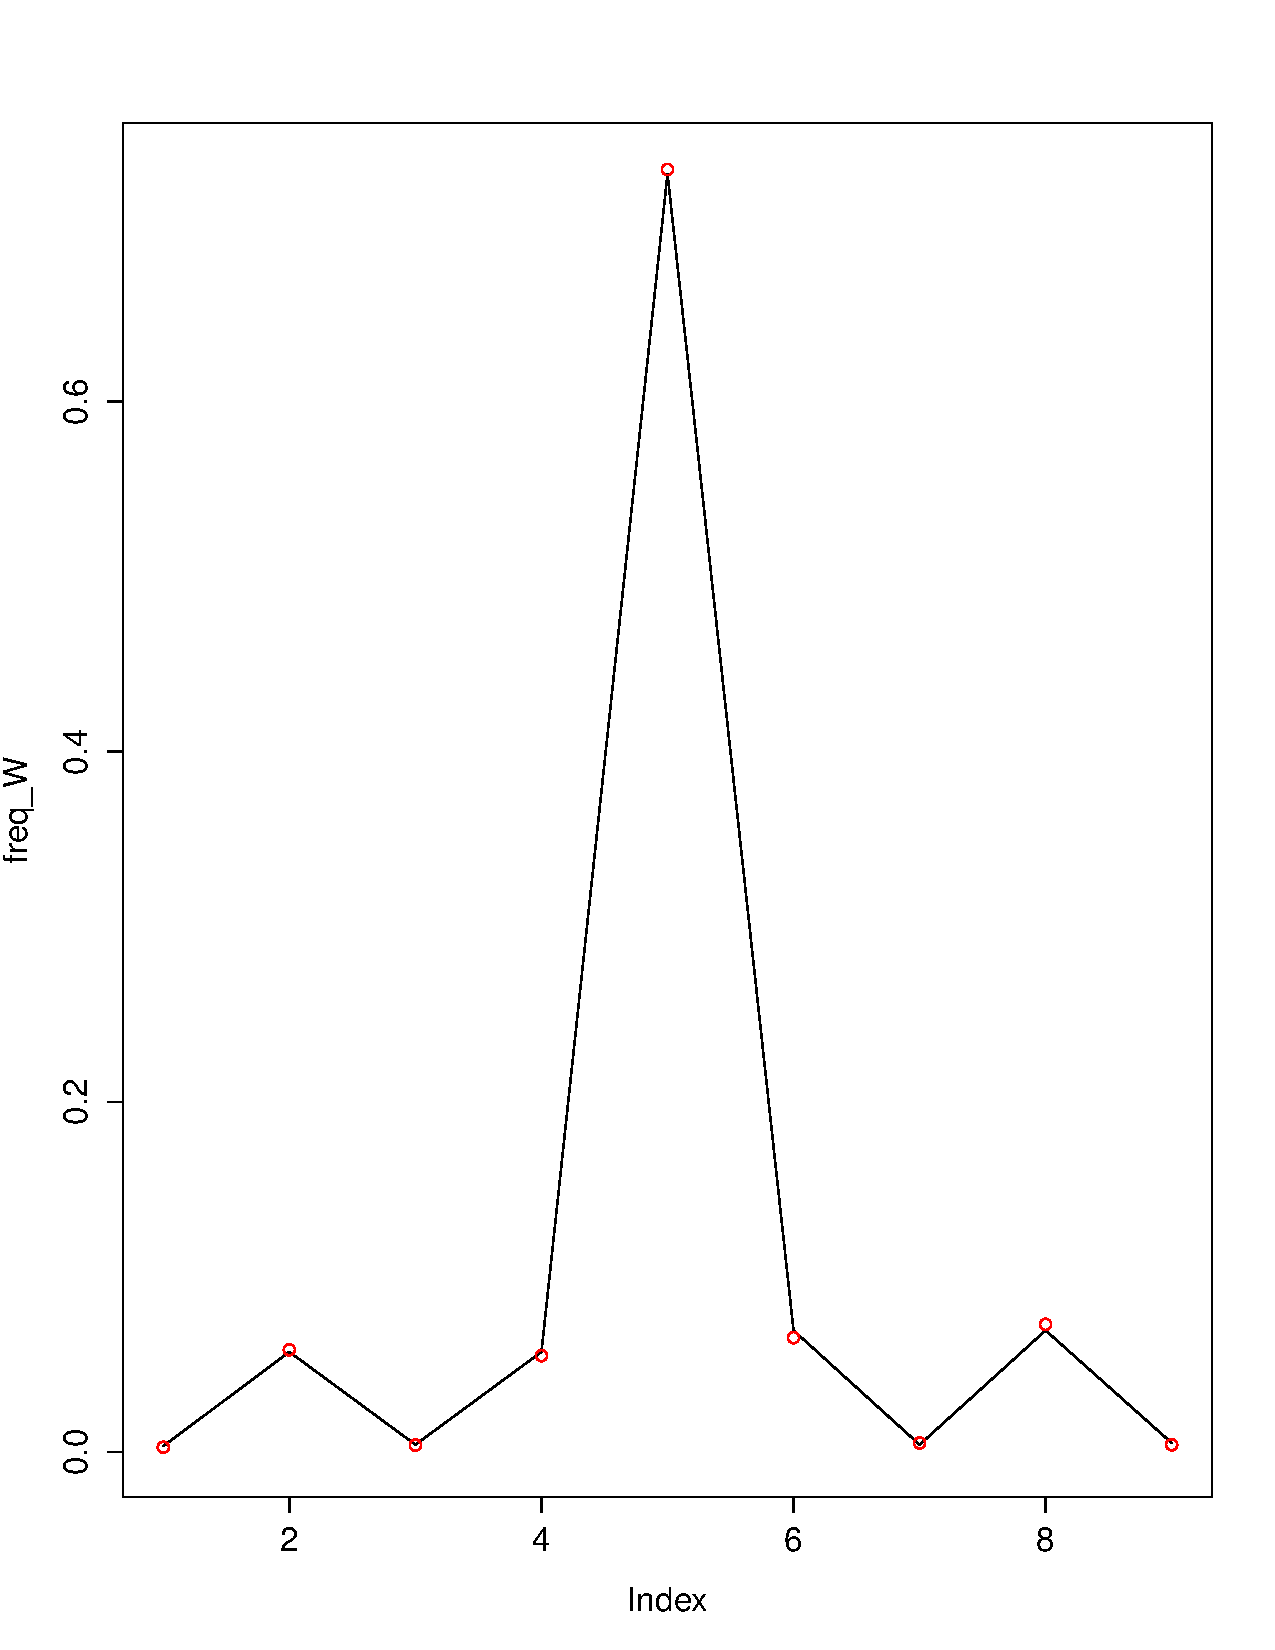
\includegraphics[scale=0.2]{freq_simple_sim.pdf}
\caption{Stationary probabilities with 2 sites}
\label{fig:freq2sites}
\end{figure}

In Figure~\ref{fig:freq2sites} on page ~\pageref{fig:freq2sites} the solid line connects the values of stationary probabilities for each state from theoretical calculation, and the red circles from simulation. \\
%Obviously the simulation is done correctly and analyzed correctly in this case.\\

\item Another simulation is done with 2 sites (3 states for each site) for each protein, starting with $(1,2)$, with optimal protein $(2,2)$, selection coefficient  0.1, running time $10^9$, sites dependent. The stationary probabilities are:
\begin{table}[here]
\begin{center}
\begin{tabular}{rrrrrrrrrr}
  \hline
  1 & 2 & 3 & 4 & 5 & 6 & 7 & 8 & 9 \\ 
  \hline
 0.003364677 & 0.057514946 & 0.004235888 & 0.058025656 & 0.727881756 & 0.069636795 & 0.004130742 & 0.070132484 & 0.005077057 \\ 
0.003324449 & 0.057134781 & 0.004132447 & 0.057134781 & 0.730153540 & 0.069429813 & 0.004132447 & 0.069429813 & 0.005127929 \\ 
   \hline
\end{tabular}
\end{center}
\end{table}

First row is from simulation, second row is from Sella-Hirsh's formula. They are very close to each other. The number of steps in this simulation is $669061$, which is relatively big.\\

\item A simulation with 3 sites and 3 states for each site confirmed the correctness of simulation. The chain starts with $(1,1,1)$, with optimal protein $(2,2,2)$, selection coefficient $0.01$, running time $10^8$, sites dependent. The number of observations is $216126$. Figure~\ref{fig:freq3sites} on page ~\pageref{fig:freq3sites} is a plot of stationary probabilities from both simulations and Sella-Hirsh's formula.
\begin{figure}[here]
\centering
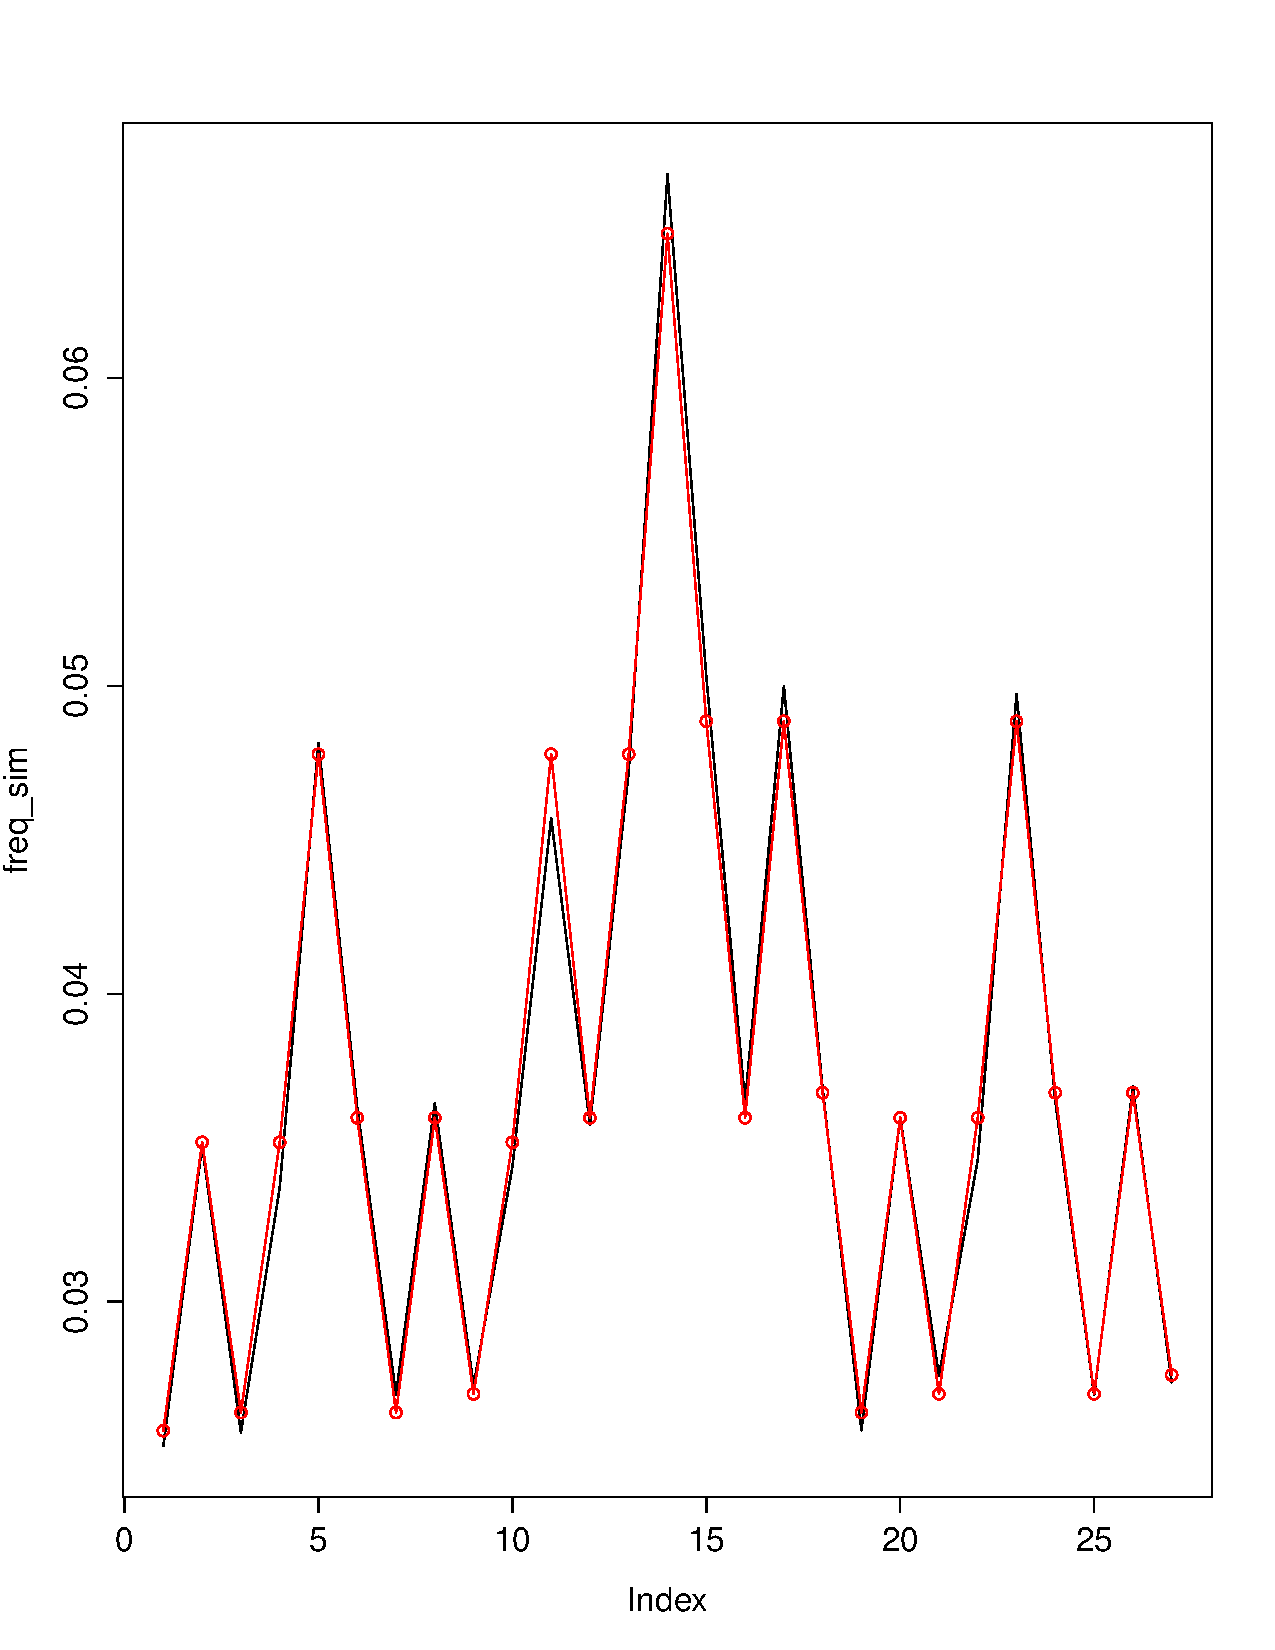
\includegraphics[scale=0.3]{3sites3states.pdf}
\caption{stationary probabilities with 3 sites}
\label{fig:freq3sites}
\end{figure}

\end{enumerate}

\begin{center}
\line(1,0){250}
\end{center}

Questions to answer next:
\begin{enumerate}
\item How to construct phylogeny from the simulated data?\\

\item How to approximate the functionality (and other variables of concern) in the site-dependent case using site-independent case?\\

In site-independent case, it's equivalent to assuming that every other site is at the optimal amino acid hence the functionality at those sites is 1. When the process has reached stationarity, if $\Phi$ is high and selection is strong, then the frequency of optimal amino acids will be high hence the assumption is reasonable. However, when $\Phi$ is small or selection is very weak, there tend to be more non-optimal amino acids at many sites.\\

Consider the case when there are only 2 sites (amino acids) in the protein, fix the second site at a certain amino acid and let only site 1 change. How does site 2 affect the stationary distribution at site 1?\\

From \eqref{eq:fitnessratio},
\begin{equation}
f_{ij} = \frac{f_i}{f_j} = \exp\Big(-\frac{A}{F_2}(e^{d_is_1} - e^{d_js_1})\Big)
\label{eq:fitratioindep}
\end{equation}
In site-independent case, we assume site 2 is at the optimal amino acid, i.e. $F_2 = 1$, therefore
\begin{equation}
f_{ij}^{\text{ind}} = \exp\Big(-A(e^{d_is_1} - e^{d_js_1})\Big)
\end{equation}

The relationship between the two fitness ratios is
\begin{equation}
f_{ij}^{\text{ind}} = (f_{ij})^{F_2}
\end{equation}

If site 2 is not at the optimal amino acid, then $F_2 < 1$. Now consider the fitness ratios between an amino acid ($aa_i$) and the optimal amino acid ($aa_o$).\\
\begin{eqnarray}
f_{io} & = & \exp\Big(-\frac{A}{F_2}(e^{d_is_1} - 1)\Big)\\
f_{io}^{\text{ind}} & = & (f_{io})^{F_2}
\end{eqnarray}
Since $f_{io} < 1$, $f_{io}^{\text{ind}} > f_{io}$, the fixation probability from an arbitraty amino acid to the optimal amino acid is higher in the site-dependent case. In other words, the selection strength at one site is {\bf higher} when other sites are not at the optimal amino acids.\\

Let's see what happens with stationary distributions under site-independent and -dependent cases. From \eqref{eq:stationary}, 
\begin{equation}
\frac{p_i}{p_o} = \big(\frac{f_i}{f_o}\big)^\nu = (f_{io})^\nu
\end{equation}
Therefore 
\begin{equation}
(\frac{p_i}{p_o})^{\text{ind}} = (f_{io}^{\text{ind}})^\nu = (\frac{p_i}{p_o})^{F_2} > \frac{p_i}{p_o}
\end{equation}

This result could easily be generalized when the functionality $F_S$ is known for othere sites and only one site is changing, with $F_2$ replaced by $F_S$. Simulations also verified the relation.\\

Rewriting the equation \eqref{eq:fitnessratio}, we can see
\begin{equation}
\frac{f_i}{f_j} = \exp\Big[-A\Big(e^{d_k^i s_k - \ln F_S} - e^{d_k^j s_k -  \ln F_S}\Big)\Big]
\end{equation}
What does this reflect the effect of $F_S$ on selection strength at site $k$?\\

The most essential and what we are most interested in are the fixation rates from one protein to another, under both site-dependent and site-independent cases. If this is clear, the substitution rates and stationary distribution will follow, also the mean fitnesses. On the other hand, fixation probability is a function of fitness ratio, which also determines the stationary probabilities.\\

Now we already know how to express the fitness ratio in site-dependent case in terms of that in site-independent case, with functionality at other sites as exponent, when there is only one site that is different between two proteins. \\

To get the fitness ratio between any two proteins, we could use proteins that are one site away from them as bridges and represent the ratio as a product of several ratios we already know. For example:

\begin{eqnarray*}
\frac{f_{AA}}{f_{BB}} & = & \frac{f_{AA}}{f_{AB}} \cdot \frac{f_{AB}}{f_{BB}}\\
\frac{f_{AA}}{f_{AB}} & = &(\frac{f^2_A}{f^2_B})^{-F_A}\\
\frac{f_{AB}}{f_{BB}} & = &(\frac{f^1_A}{f^1_B})^{-F_B}
\end{eqnarray*}

If furthermore, the selection coefficients at the first and second positions are the same, then $\frac{f^2_A}{f^2_B} = \frac{f^1_A}{f^1_B} = \frac{f_A}{f_B}$ in site-independent case. Therefore
\begin{equation*}
\frac{f_{AA}}{f_{BB}} = (\frac{f_A}{f_B})^{-F_A-F_B}
\end{equation*}

If there are more than 2 sites that are different, then there need to be more than one intermediate proteins to relate them together. For example,
\begin{equation*}
\frac{f_{AAA}}{f_{BBB}} = \Big(\frac{f_A}{f_B}\Big)^{-F_{AA}-F_{AB}-F_{BB}}
\end{equation*}
However, if the selection coefficients are not the same across the sites, this relationship does not hold any more. The reason is that even fitness ratio in site-independent case depends on the selection coefficient at that particular site. 
\end{enumerate}
%Next step: set the mutation rate to be a different number, add mutation bias, move from amino acid level to codon level.

\begin{center}
\line(1,0){250}
\end{center}

Parameters to investigate during the optimization (optimx):\\
\begin{enumerate}
\item $s, \Phi, C, q, N_e$, some of them are correlated to each other and cannot be split separately
\item tree topologies (at different extremes), branch lengths, number of tips
\item ancestral sequences --- stationary, uniform, same sequence as used in the simulation
\end{enumerate}

Hessian matrix, variance, information; confidence interval, bootstrapping; ...

\begin{center}
\line(1,0){250}
\end{center}

Meeting on Thursday, Mar 8, 1012.
\begin{enumerate}
\item Do the plots of MLE bias with respect to number of sites (200, 400, 800 or more in between) : first, fix other parameters, estimate $s$; second, estimate $\Phi$ while fix other parameters. Do this for trees with 4 tips and 8 tips.
\item Estimate the composite parameter.
\item Instead of giving the equilibrium frequencies, make it depend on the parameters as from Sella-Hirsh's formula, and do the optimization that way.
\item Let $s$ vary according to Gamma distribution instead of being fixed, and estimate the Gamma parameter(s).
\end{enumerate}

Profiling R code:

> Rprof(file="rprof.out")
> R command
> Rprof(NULL)

under unix, use command:
R CMD Rprof rprof.out
\end{document}
